% !TeX root = ../../main.tex
\section{Non-detailed reactor modelling} \label{Non-detailed}

The reactors were chosen on the basis of safety and performance. For the hydrogenation of ONT, a co-current trickle bed reactor was chosen due to the high conversion performance and absence of moving parts that might damage the expensive Pd/C catalyst. The high pressure required for the reaction can also be well controlled in a trickle bed reactor. 

Fluidised bed reactors were initially considered for the oxidation and hydrogenation of PNT derivatives, but were ruled out considering the attrition of catalyst particles due to the high flowrates. Packed-bed reactors were chosen and optimised to address its limitation of concentration and temperature gradients by controlling the residence time. Full detailed analysis for each reactor choice can be found in Section \ref{sec:reactorchoices}.

\begin{table}[h]
\centering
\caption{Summary of non-detailed reactors}
\label{tab:nondetailedtable}
\resizebox{\textwidth}{!}{%
\begin{tabular}{@{}llllllll@{}}
\toprule
Tag  & Type & Process & \splitcell{Volume\\ (\si{\cubic\m})} & Temperature (K) & Pressure (atm) & Duty (kW) & Conversion \\ \midrule
R201 & Co-current trickle bed & Hydrogenation & 3.93 & 333 & 5 & -137.78 & 98\% \\
R301 & Packed-bed & Oxidation & 0.02 & 750 & 1 & -77.20 & 62\% \\
R401 & Packed-bed & Oxidation & 2.75 & 750 & 1 & -56.25 & 100\% \\
R501 & Packed-bed & Hydrogenation & 0.70 & 298 & 1 & -125010 & 80\% \\
R601 & Packed-bed & Hydrogenation & 0.60 & 298 & 1 & -73.80 & 86\% \\ \bottomrule
\end{tabular}%
}
\end{table}

\subsection{R201: Hydrogenation of o-nitrotoluene}
After the production of the 3 nitrotoluene isomers, (mention separation?) ONT is mixed with propanol and hydrogenated to o-TOL in a co-current trickle bed reactor operating at 333K and 3 atm. 

\begin{scheme}[h]
    \centering
    \ch{ ONT + 3 H2 -> O{-}TOL + 2 H2O }
    \caption{ONT hydrogenation to O-TOL}
    \label{eqn: ONT hydrogenation}
\end{scheme}

include ChemDraw here
The rate equation for this equation can be defined as: 
\begin{equation}
    r = k P_{H_2}^{0.3} 
    \label{ONT rate equation}
\end{equation}
 \begin{equation}
    k = 211.69 \exp \left(-\frac{45.52 \cdot 10^{3}}{RT}\right) ~(\si{\mol\per\kPa\tothe{0.3}\per\g\of{cat}\per\s})
 \end{equation}
 
\subsection{R301 \& R401: Oxidation of p-nitrotoluene}
% Andreas

The oxidation of p-nitrotoluene is performed in packed-bed reactors R301 and R401, employing air as the oxidant. The overall reaction network is shown in \cref{sch:R3} and is based on that reported for the oxidation of toluene \cite{hoorn_modelling_2005}. Kinetic information was sourced for the toluene oxidation network and corrected for the deactivation effect of the nitro- substituent using Hammett constants, giving rates for the nitrotoluene network 5.6 times slower than  \cite{partenheimer_methodology_1995}. These data are shown in \cref{tab:S3-kinetics}. The rate expression for each step does not depend on the concentration of \ch{O2}
\begin{scheme}[h]
    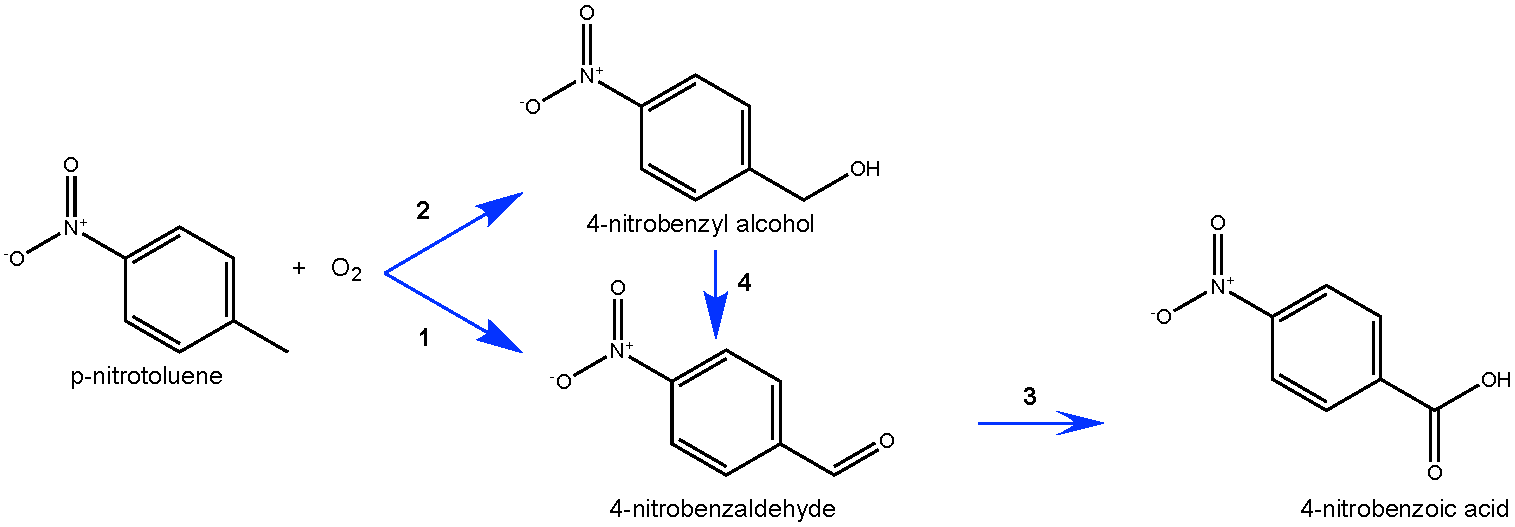
\includegraphics[width=\linewidth]{figures/R3.pdf}
    \caption{Oxidation of 4-nitrotoluene to 4-nitrobenzaldehyde, and subsequently to 4-nitrobenzoic acid}
    \label{sch:R3}
\end{scheme}

\begin{table}[h]
\centering
\caption{Corrected kinetic data for the oxidation network \cite{tan_kinetic_2010}}
\label{tab:S3-kinetics}
\begin{tabular}{@{}lS[table-format=1.3e1]S[table-format=3.2]@{}}
\toprule
Reaction & {$A$ (\si{\per\s})} & {$E_a$ (\si{\kJ\per\mol})} \\ \midrule
1        & 7.068e9  & 123.91      \\
2        & 1.503e3  & 69.54       \\
3        & 5.621e4  & 66.84       \\
4        & 3.384e6  & 81.27       \\ \bottomrule
\end{tabular}
\end{table}

\subsection{R501 \& R601: Hydrogenation of nitrobenzaldehyde and nitrobenzoic acid}

\begin{scheme}[h]
    \centering
    \ch{ NBA + HCOOH -> ABA + CO2 + H2O }
    \\
    \ch{ NBAH + HCOOH -> ABAH + CO2 + H2O }
    \caption{Hydrogenation of NBA and NBAH to ABA and ABAH}
    \label{eqn: ONT hydrogenation}
\end{scheme}

The hydrogenation of p-nitrobenzaldehyde and p-nitrobenzoic acid were carried out in methanol solvent with formic acid as the reducing agent. The reaction was carried out at room temperature and 1 atm. 5\% w/w Pt/C was chosen as the desired catalyst to speed up the reaction because it can be reused many times while maintaining its catalytic performance \cite{rahman_fast_2020}. The overall yield for 4-ABA and 4-ABH are 86\% and 80\% respectively as reported in [gowda and mahesh].

